\section{Problem 2A: Deterministic SIR model}

\subsection{a)}

The ODE-solver I chose to use is the one I made for exercise $2$, as I am very familiar with this, and found it working reasonably good for these kind of purposes. The implementation is an object-oriented version of the solver methods shown in the lectures and should be easily understood by the documentation in \lstinline|ode.py|.

I solve the deterministic SIR equations in terms of fractions of people. As seen in figure \ref{fig:SIR} the asymptotic expressions for $S(t)$ and $R(t)$ as given in the exam-sheet \cite{sheet}. The expressions for $S(\infty)$ and $R(\infty)$ are solved using the non-linear equation solver \lstinline|fsolve| from \lstinline|scipy|, with initial guesses $0.5$ for both.

\begin{figure}[htb]
	\centering
	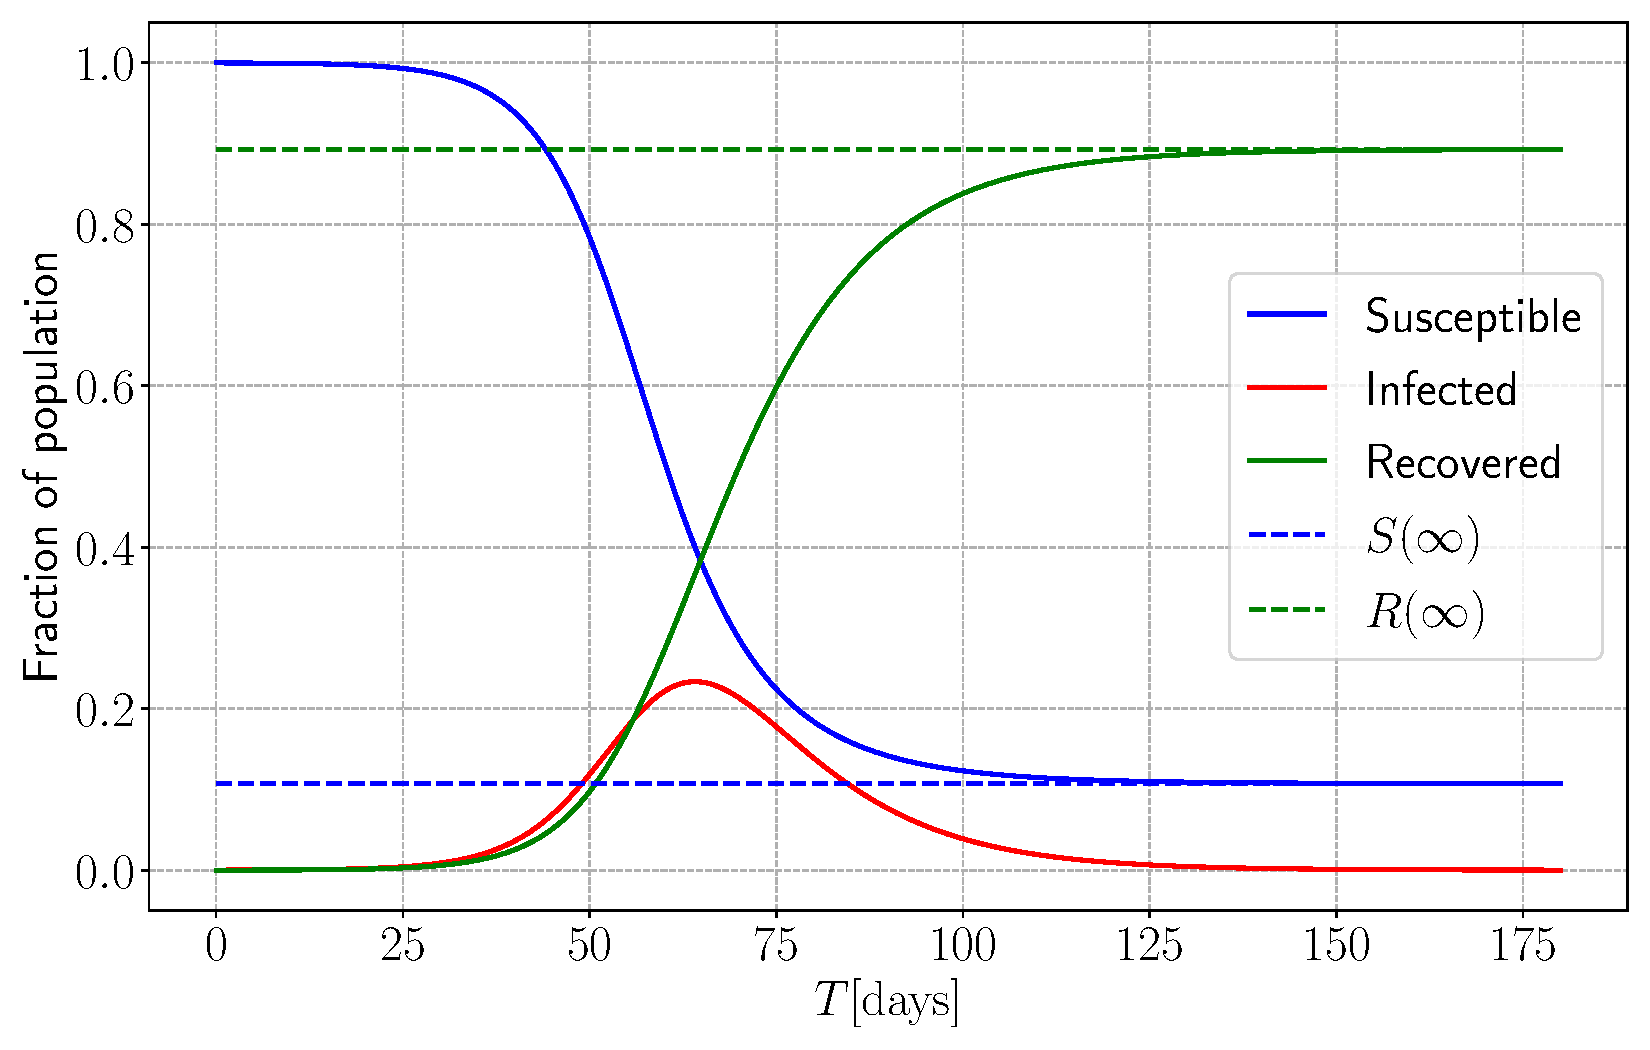
\includegraphics[width=0.8\columnwidth]{../fig/2Aa_SIR.pdf}
	\caption{SIR equations with $\beta = 0.25 \, \mathrm{day}^{-1}$, $\tau = 10 \, \mathrm{day}$.}
	\label{fig:SIR}
\end{figure}

\subsection{b)}

For the early developments of the epidemic, the expression for $I$ can be simplified to \cite{sheet}
\begin{equation}\label{eq:I_simp}
	\der{I}{t} = (\beta - 1/\tau) I.
\end{equation}
The solution of this equation is given by
$$
	I(t) = I(0) \exp{\left(\left[ \beta \tau - 1 \right] \frac{t}{\tau}\right)} = I(0) \exp{\left(\left[ \mathcal{R}_0 - 1 \right] \frac{t}{\tau} \right)},
$$
where we have introduced $\mathcal{R}_0 = \beta\tau$. As seen in figure \ref{fig:Infected}, the fraction of infected people matches this expression quite closely during the first $40$ days or so. This confirms the exponential growth in the beginning. 

\begin{figure}[htb]
	\centering
	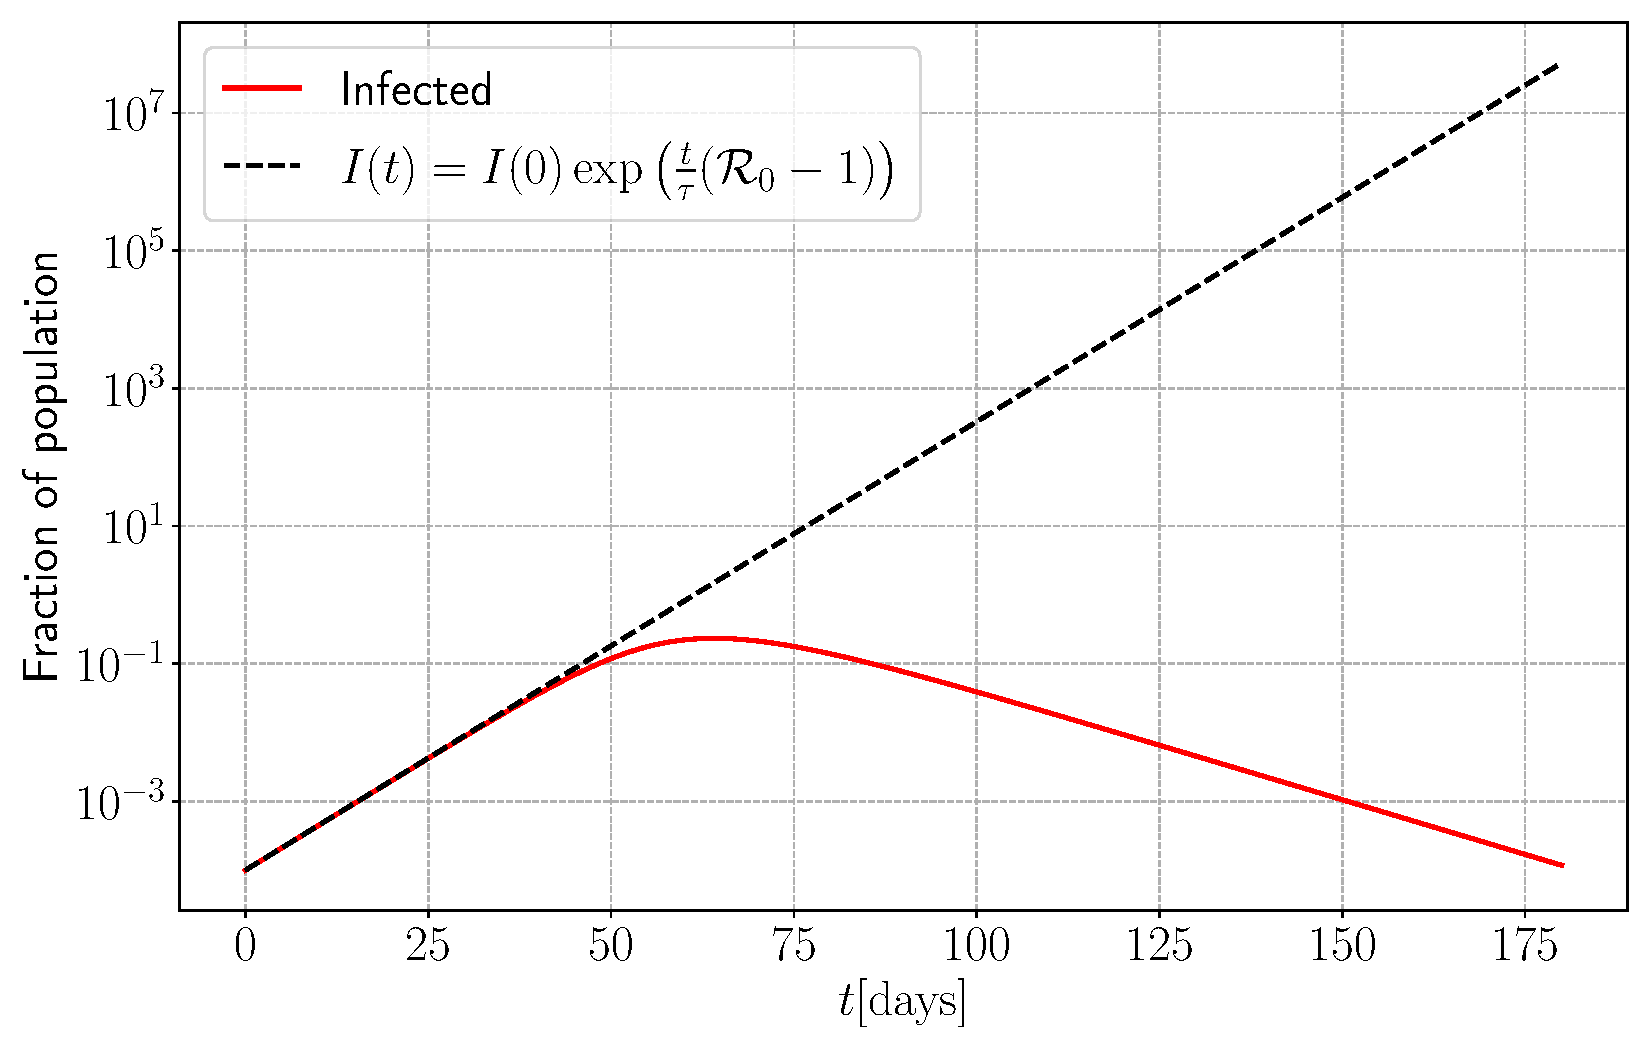
\includegraphics[width=0.8\columnwidth]{../fig/2Ab_I.pdf}
	\caption{Infected people compared with the analytical approximation at the early stages.}
	\label{fig:Infected}
\end{figure}

\subsection{c) Flattening the curve. }

As seen from figure \ref{fig:SIR}, the peak of the infected people is rather close to being at $0.2$ when $\beta = 0.25$. Remark also that the peak occurs in the early stage of the epidemic. We use these observations to our favour when finding the \textit{largest} $\beta$ that will keep $I/N$\footnote{Note that I use fractions of people instead of actual numbers of people in this section, so that is why I refer to $I$ as if it is $I/N$ in the procedure below.} smaller than $0.2$ during the pandemic. To do this, I choose the following procedure:

\begin{algorithm}[H]
	Choose a starting value for $\beta = \beta_0$\;
	Choose a tolerance $\texttt{tol}$\;
	Run the simulation of the SIR with the same parameters as in 2Aa, except with $\beta = \beta_0$.\;
	Calculate $\mathcal{I} \coloneqq \max_{t\in[0,180]} I(t)$.\;
	\While{\texttt{err }$\coloneqq | \mathcal{I} - 0.2 | > \texttt{tol}$}{
		\eIf{
			$\mathcal{I} > 0.2$
			}
			{$\beta\gets \beta \cdot 2^{\texttt{err}}$}
			{$\beta\gets \beta \cdot 2^{-\texttt{err}}$}	
		}
		Run the simulation of the SIR with the same parameters as in 2Aa, except with the new value for $\beta$.\;
		Recalculate $\mathcal{I} \coloneqq \max_{t\in[0,180]} I(t)$.\;
	\caption{Finding the largest beta keeping $\max I$ \textit{less} than 0.2.}
\end{algorithm} 

This procedure is by no means any advanced piece of algorithm, but it ensures that $\beta$ is increased when the maximum of $I$ is less than $0.2$, and decreased when it is larger than $0.2$. Further, it also ensures that the "nudging" of beta in each step is less when the error is less. To get an estimate for the \textit{largest} $\beta$ one can have to keep $I/N$ \textit{less} than $0.2$, one should start off with an initial value $\beta_0$ for which the peak is less than $0.2$, so that one reaches the limit from below. Using $\beta_0 = 0.2$, one finds with the maximum value of $\beta = 0.28020370$, as given in table \ref{tab:2Acd} together with the deviation $0.2 - \max_{t\in[0,180]} I(t)$ this value gives rise to.  


%\begin{figure}[htb]
%	\centering
%	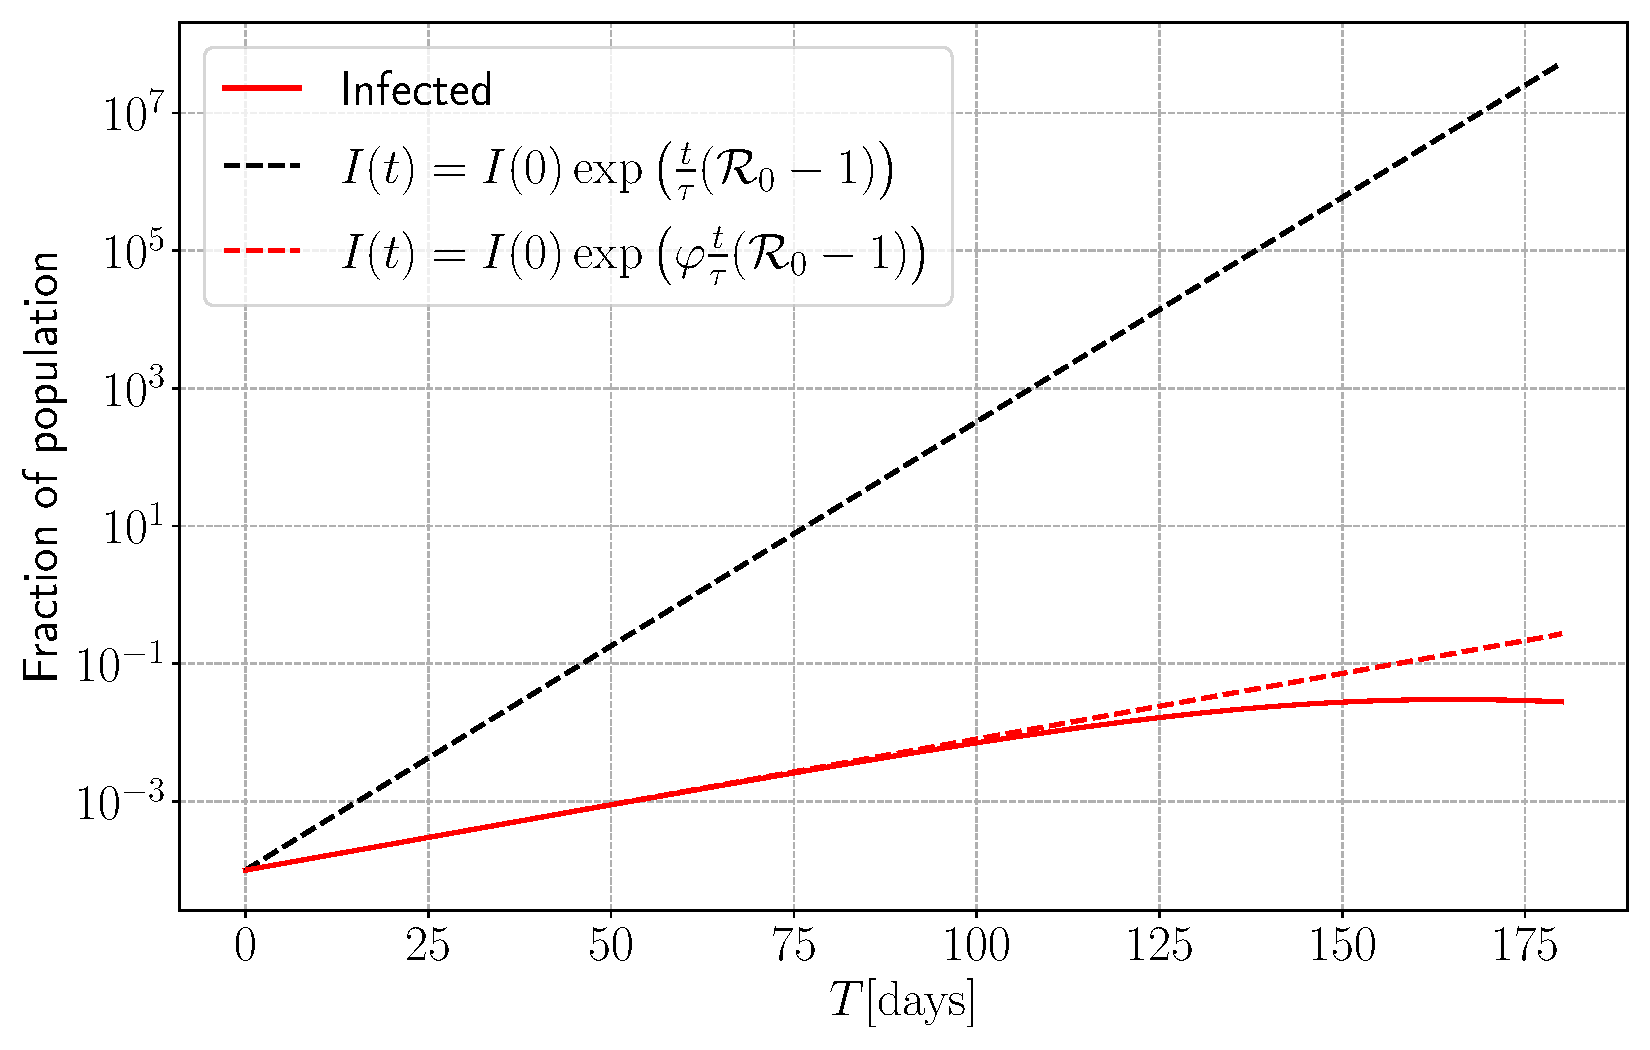
\includegraphics[width=0.8\columnwidth]{../fig/vac.pdf}
%	\caption{The effect of vaccination, with $\varphi = 0.3$.}
%	\label{fig:vaccination}
%\end{figure}

\subsection{d) Vaccinations}

To find the minimum fraction of vaccinated people preventing an outbreak, $R(0)/N$, I use the following procedure:

\begin{algorithm}[H]
	Choose a starting value for $R(0) = R_0$\;
	Run the simulation of the SIR with the same parameters as in 2Aa, except with $R(0) = R_0$ \;
	Calculate the \texttt{slope} of the fraction of infected people in a semi-log plot for the first $15$\footnote{As people are typically sick for $10$ days ($\tau = 10$) I regard this time scale as long enough to detect whether the outbreak grows exponentially or decays.} days of the simulation\;
	If the initial slope is negative it indicates that the outbreak dies out by itself\;
	\While{\texttt{slope}$ > 0$}{
		$R(0) \gets R \cdot 2 ^{\texttt{slope}}$ \;
	Run the simulation of the SIR with the same parameters as in 2Aa, except with the new value for $R(0)$.\;
	Recalculate the \texttt{slope} in the semi-log axes.\;}
	\caption{Finding the minimum fraction of initially vaccinated people for outbreaks to be impossible.}
\end{algorithm} 

The value of $R(0)/N$ preventing an outbreak found from this procedure is $0.59987499$, as shown in table \ref{tab:2Acd} together with the slope in the semi-log plot which this fraction yields for $I(t)$. This is obtained from running the procedure with $R_0 = 0.1$.

\begin{table}[htb]
	\centering
	\caption{The maximum value of $\beta$ giving a peak less than $0.2$ of the infected fraction, and the minimum value of $R(0)$ (vaccinated) avoiding exponential growth.}
	\begin{tabular}{cccc}
		\toprule
		Parameter & value & $0.2 - \max_{t\in[0,180]} I(t)$ & Initial $\log$-slope \\
		\midrule
		$\beta$ & $0.28020370$ & $8.319\cdot 10^{-7}$ & --- \\
		$R(0)$  & $0.59987499$ & --- & $-1.74\cdot 10^{-15}$ \\
		\bottomrule
	\end{tabular}
	\label{tab:2Acd}
\end{table}


\clearpage
